
%(BEGIN_QUESTION)
% Copyright 2014, Tony R. Kuphaldt, released under the Creative Commons Attribution License (v 1.0)
% This means you may do almost anything with this work of mine, so long as you give me proper credit

Calculate the lower and upper range values for this level transmitter, given the information in the following diagram.  Assume the ``low'' side of the transmitter is vented to atmosphere.  Be sure to provide your answers in units of inches water column ("W.C.):

$$\includegraphics[width=15.5cm]{i02555x01.eps}$$

LRV = \underbar{\hskip 50pt} "W.C. \hskip 100pt URV = \underbar{\hskip 50pt} "W.C.

\underbar{file i02555}
%(END_QUESTION)





%(BEGIN_ANSWER)

LRV = \underbar{\bf 31.72} "W.C. \hskip 100pt URV = \underbar{\bf 158.6} "W.C.

%(END_ANSWER)





%(BEGIN_NOTES)

{\bf This question is intended for exams only and not worksheets!}.

%(END_NOTES)



